\chapter{Experimental Setup}
\label{chap:experiment}

\section{APP Setup}

\begin{figure}
    \centering
    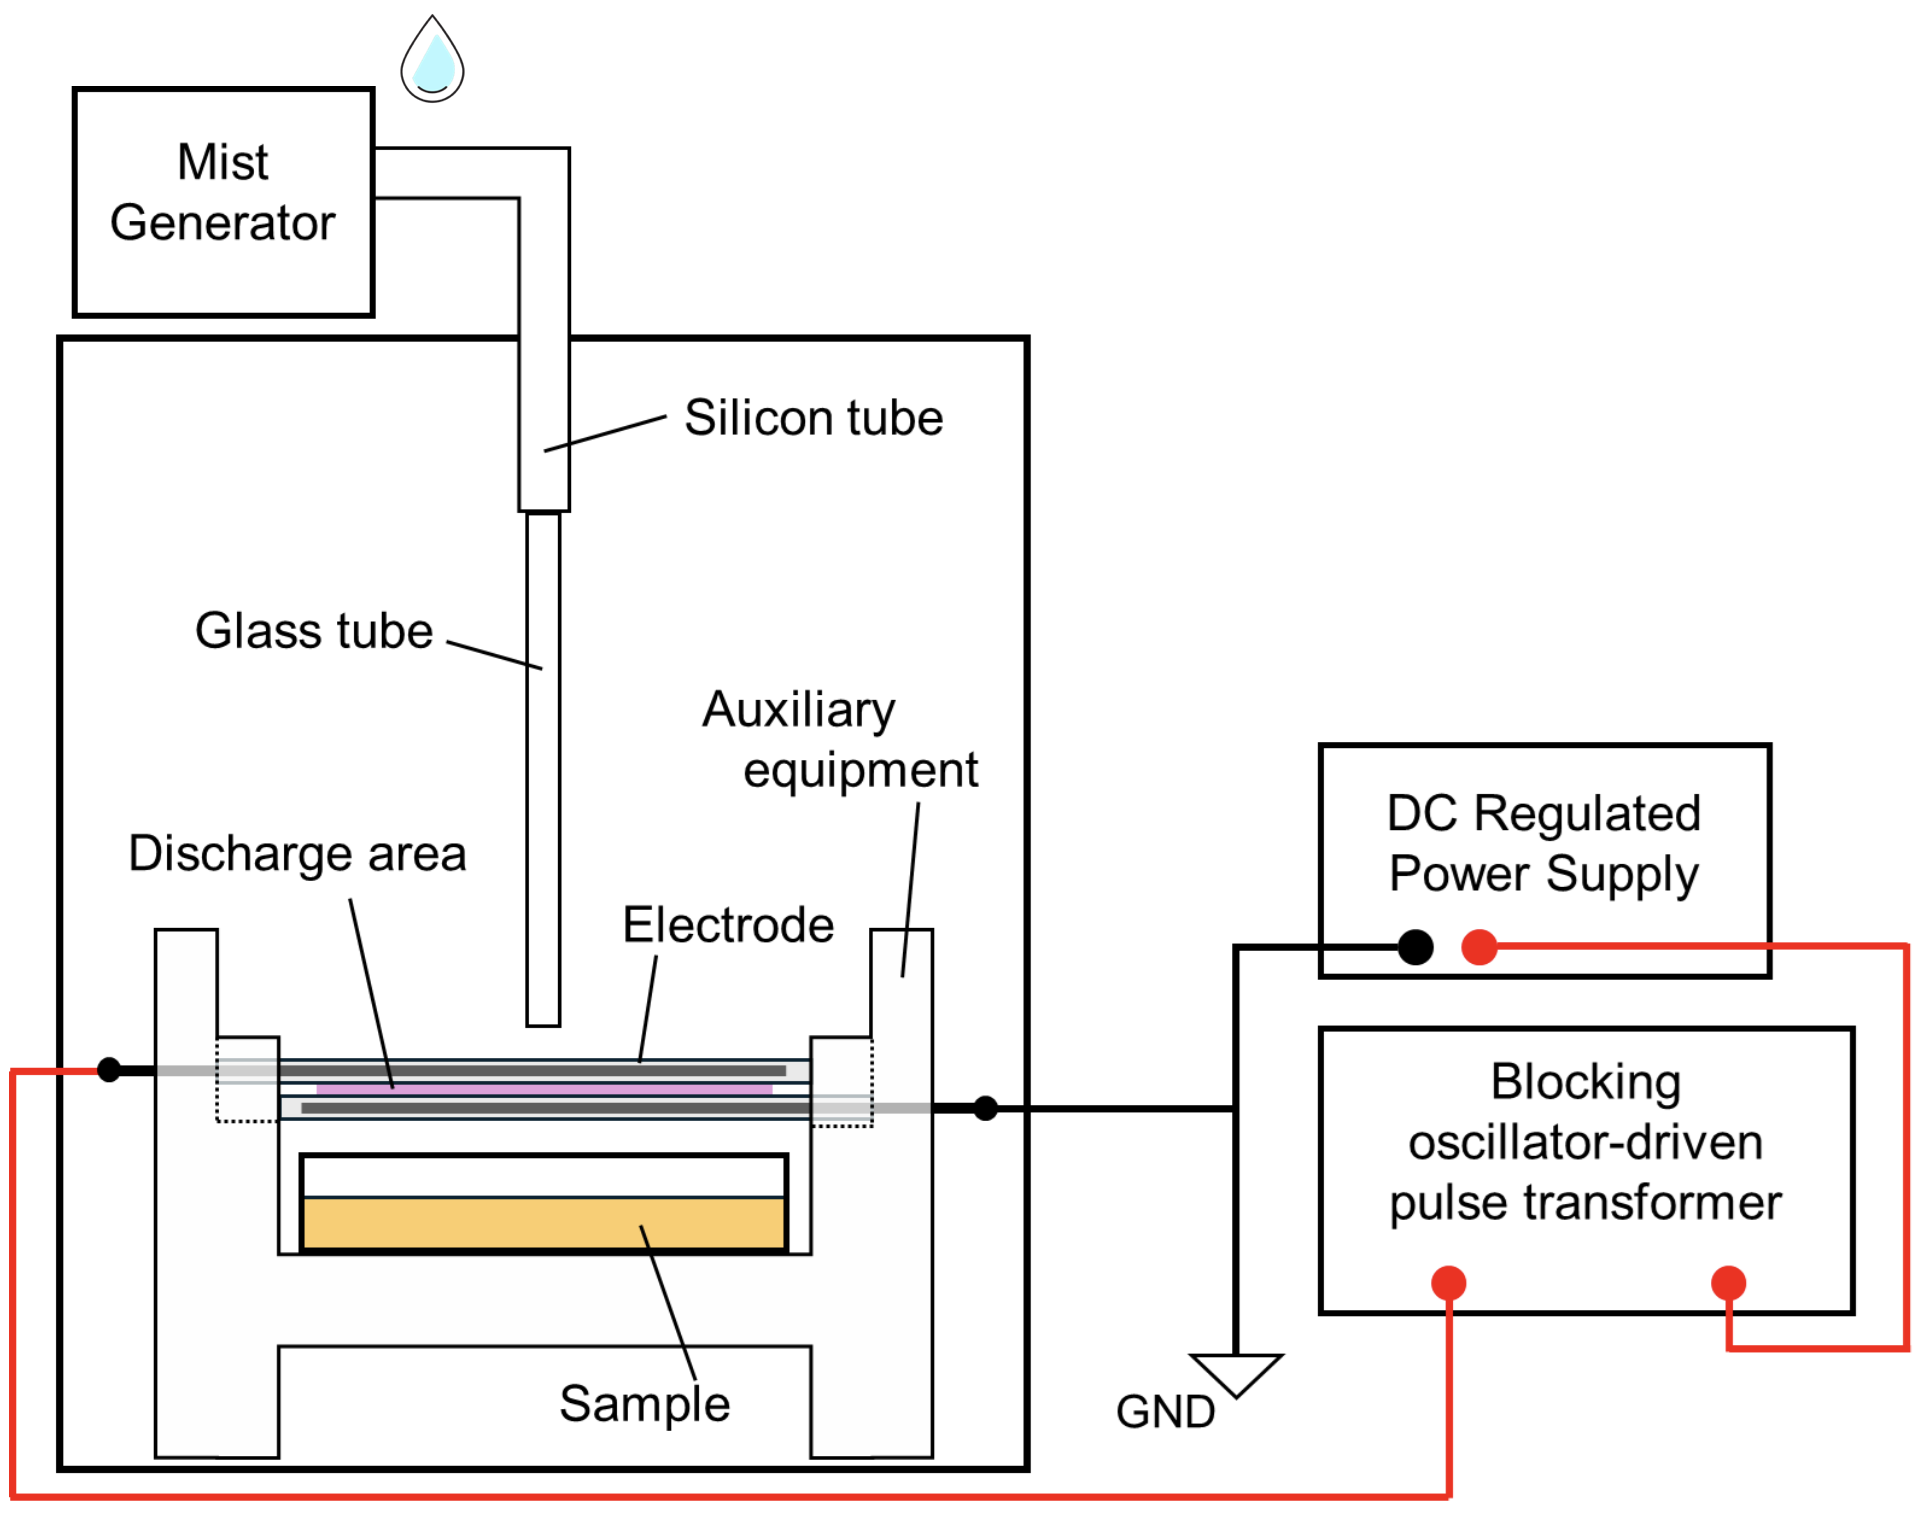
\includegraphics[width=1\textwidth]{images/Process_setup.png}
    \caption[Experimental setup]{This figure shows the experimental setup. The APP is generated between two pairs of electrodes. The entire setup is placed in a box to prevent contamination. The sample is placed underneath the discharge area. A tube can provide water mist and dry air to control the humidity in the chamber. A power supply and a blocking oscillator provide an oscillating voltage to the electrodes.}
    \label{fig:setup}
\end{figure}

\subsection{Dielectric Barrier Discharge}
\begin{figure}
    \centering
    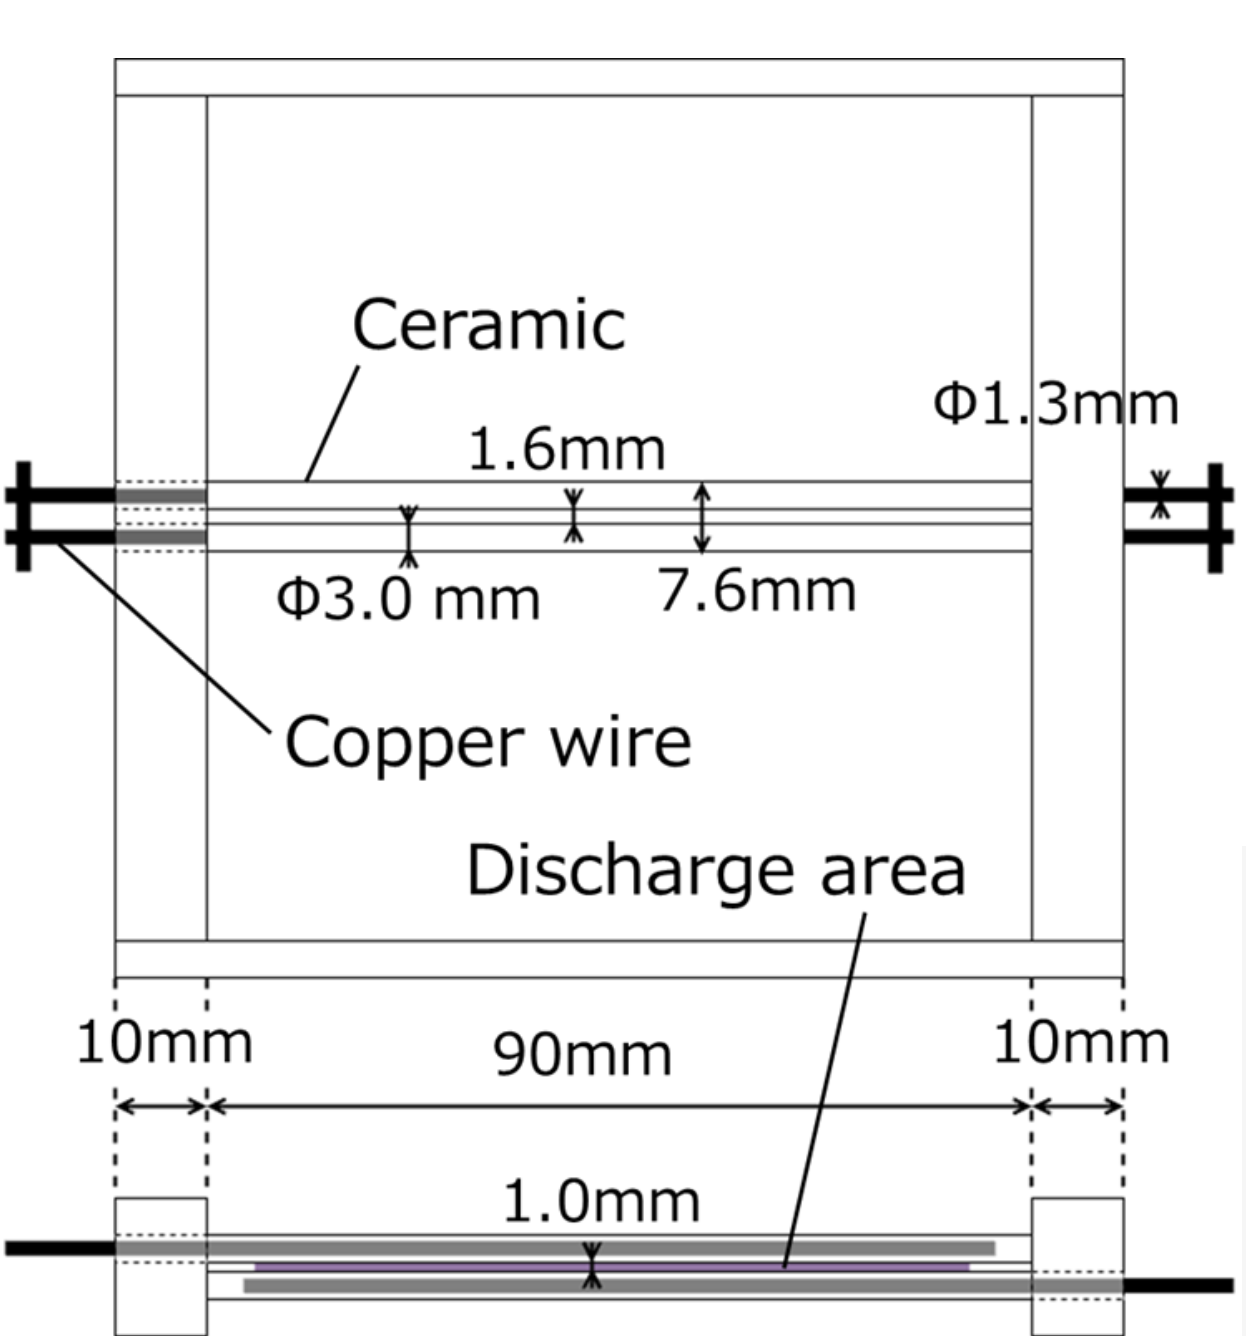
\includegraphics[width=.8\textwidth]{images/APP_setup.png}
    \caption[Technical sketch of the DBD setup]{Technical sketch of the DBD setup. On the top the view from above the DBD setup is shown, on the bottom the side view. The APP is generated by a DBD with a frequency of 13.56 MHz and a voltage of 13 kV. This diagram has kindly been provided by Shinano Kinoshita at KIT.}
    \label{fig:dbd}
\end{figure}

\begin{figure}
    \centering
    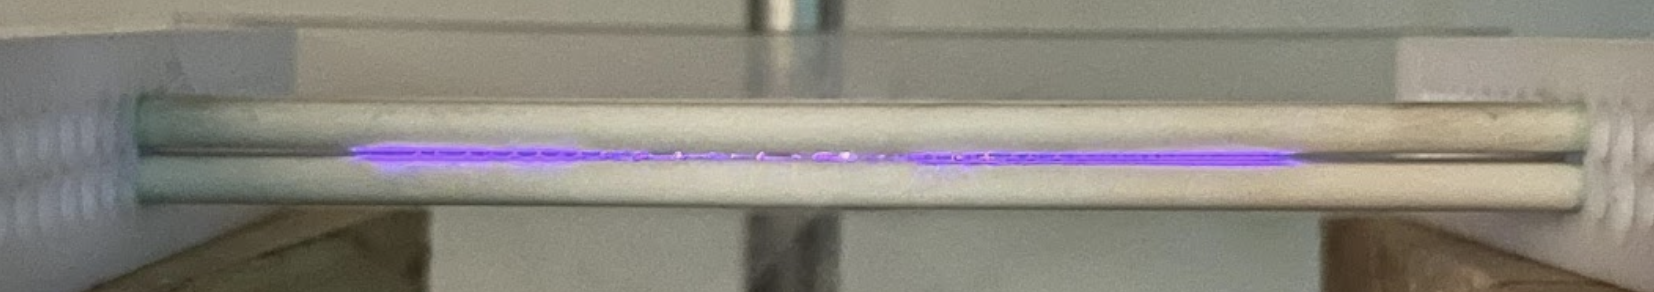
\includegraphics[width=1\textwidth]{images/Plasma.png}
    \caption[Image of the APP]{Image of an ignited plasma at atmospheric pressure between the electrodes.}
    \label{fig:plasma}
\end{figure}


\subsection{Optical Emission Spectroscopy}

\section{Preparation of Samples}
\begin{figure}
    \centering
    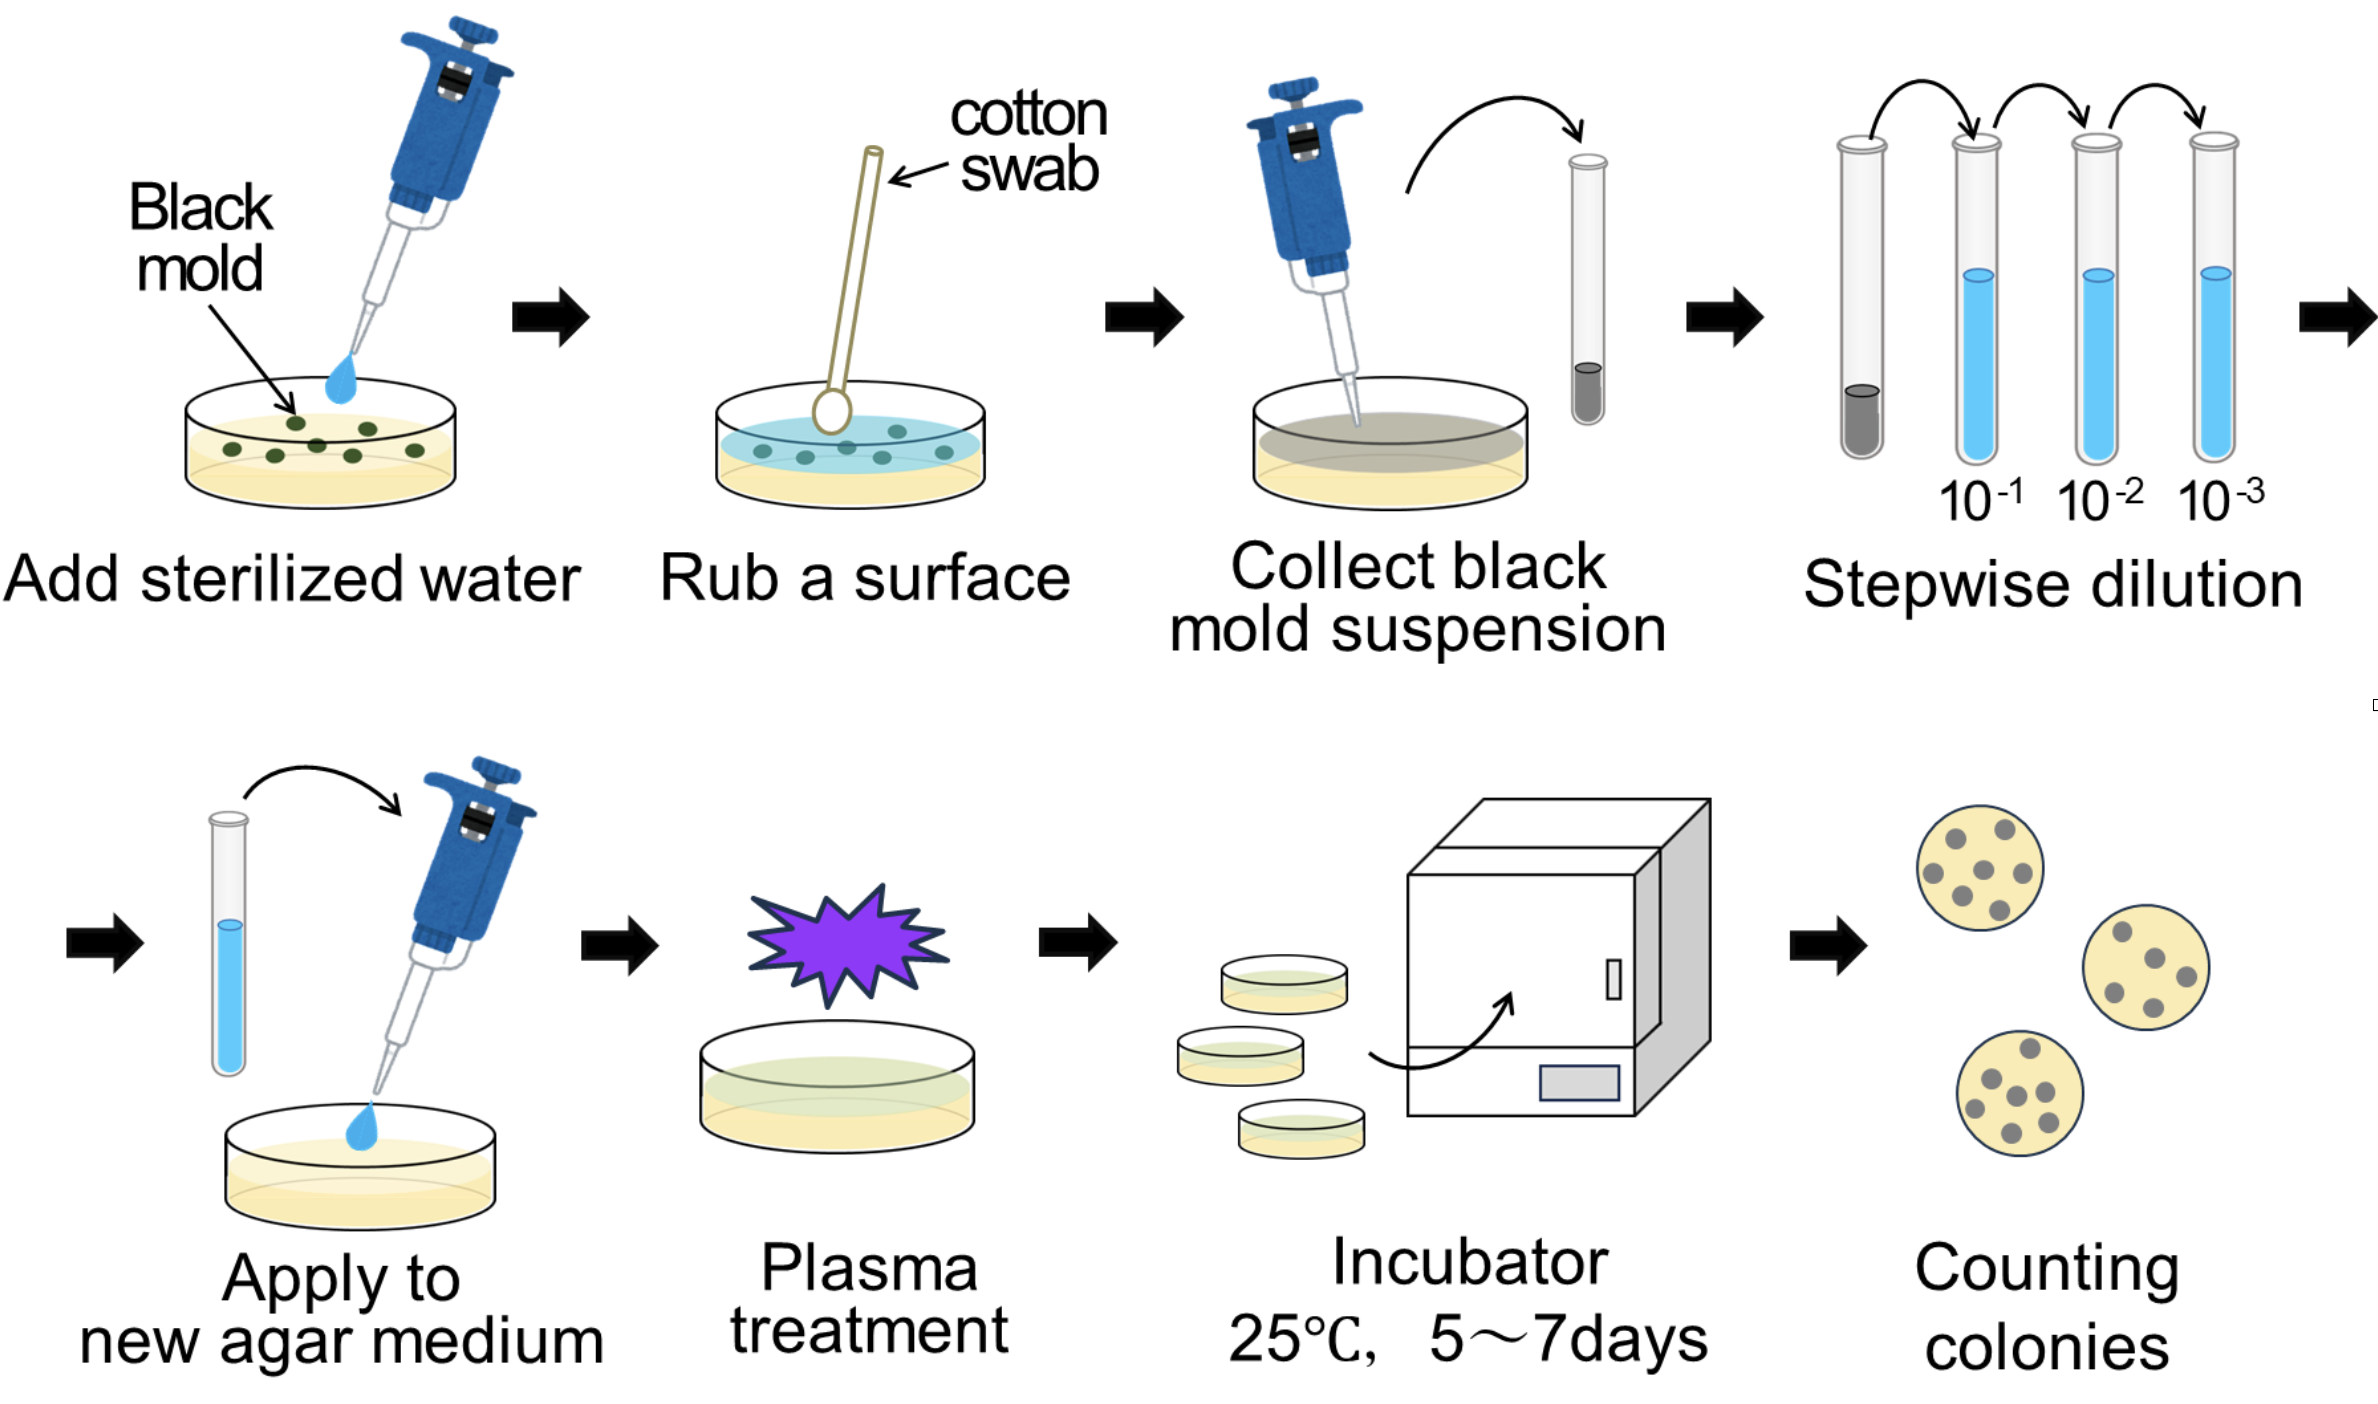
\includegraphics[width=1\textwidth]{images/Process.png}
    \caption[Diagram of the experiment process]{Diagram of the experiment process and the preparation of samples. The fungus is cultivated on an agar medium and stored in petri dishes. Spores are collected by dissolving them in sterilized water and then their concentration is diluted in steps to the desired concentration. The samples are then treated with the APP and the inactivation rate is measured by counting the colonies on the agar medium.}
    \label{fig:process}
\end{figure}

\section{UV Exposure}

\section{Plasma Treatment}

\subsection{Full Plasma Treatment}
\subsection{Isolation of Radiation}


